% *******************************************************************************
% * Copyright (c) 2007-2008 by Elexis
% * All rights reserved. This document and the accompanying materials
% * are made available under the terms of the Eclipse Public License v1.0
% * which accompanies this distribution, and is available at
% * http://www.eclipse.org/legal/epl-v10.html
% *
% * Contributors:
% *    G. Weirich - initial implementation
% *
% *  $Id: customize.tex 4896 2009-01-02 08:23:59Z rgw_ch $
% *******************************************************************************
% !Mode:: "TeX:UTF-8" (encoding info for WinEdt)

\section{Principe de fonctionnement}
La caractéristique frappante de Elexis est sa grande flexibilité. Si vous êtes habitué à un
autre logiciel, l'utilisation de Elexis peut vous apparaître un peu inhabituel. Pour cette raison nous allons tout d'abord expliquer quelques concepts de base.

\index{Principe de fonctionnement}
 \subsection{Bureau / Perspective}
 \index{Perspective}\index{Affichage}\index{View}
Imaginez votre table de travail. Vous vous êtes probablement habitué de poser certaines choses à un endroit spécifique sur votre bureau, c'est-à-dire attribuer certaines fonctions de travail à un lieu, où vous pouvez (idéalement) les retrouver facilement. Votre ordre n'est pas nécessairement le même que pour quelqu'un d'autre qui a le même modèle de bureau.
La fenêtre du programme Elexis est comme un bureau (voir fig. \ref{fig:tour1}. Il n'est en aucun cas préfixé à quel endroit une fonction spécifique doit être située et il n'est même pas définie,
lesquels des éléments doivent apparaître sur le bureau et lesquels peuvent rester rangés quelque part dans un tiroir pour être sortis seulement en cas de besoin.


%\usepackage{graphics} is needed for \includegraphics
\begin{figure}[htp]
\begin{center}
  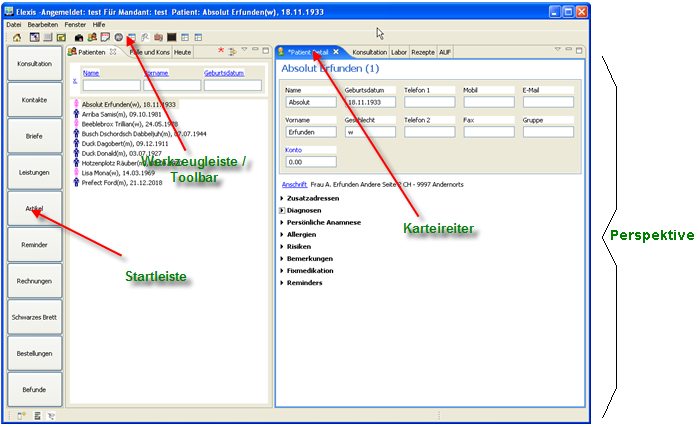
\includegraphics[width=0.9\textwidth]{images/tour1}
  \caption{Standard-Perspektive}
  \label{fig:tour1}
\end{center}
\end{figure}

Un aménagement de surface de travail nous appelons une 'perspective' (perspective). On appelle 'Affichage' (view) les différentes sous-fenêtres respectivement les sous-unités (comme en haut 'patients' et 'détails du patient') qui composent la perspective.

\subsubsection{Perspectives et views}

La (fig. \ref{fig:tour1} montre un exemple de perspective appropriée pour un petit écran.
Il affiche une capture d'écran sur un TFT 15 pouces. Les affichages \glqq
patients\grqq{}(à gauche) et \glqq détails du patient\grqq{}(à droite) se trouvent au-dessus d'autres affichages dont on ne voit que les onglets.

Sur un écran plus grand on favoriserait probablement un autre aménagement : fig. \ref{fig:tour2} montre une capture d'écran sur un TFT 17 pouces avec plusieurs views en même temps.

%\usepackage{graphics} is needed for \includegraphics
\begin{figure}[htp]
\begin{center}
  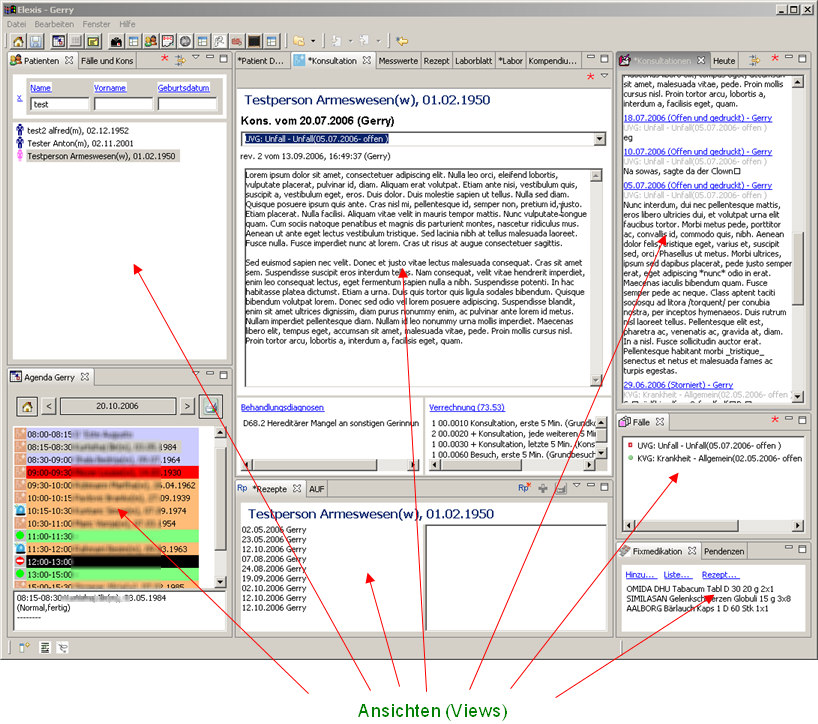
\includegraphics[width=0.9\textwidth]{images/tour2}
  \caption{Komplexere Perspektive}
  \label{fig:tour2}
\end{center}
\end{figure}

\subsubsection{Affichage / views}
Chaque affichage correspond à une fonctionnalité spécifique. Dans cette fenêtre (fig. 4.2)
on voit une liste de patients (à gauche) et les 'détails du patient' actuellement actif (à droite).
Il y a d'autres affichages comme 'Consultation' qui permet l'introduction des informations médicales dans le dossier du patient, 'l'Historique' qui est un listing de toutes les notes faites dans le dossier du patient, la 'Médication fixe', les 'Ordonnances', les 'Certificats' d'incapacité de travail, 'l'Agenda' et autres.
Chaque affichage est une  \glqq vue\grqq définie sur des données existantes. Il peut être activé en cliquant sur l'onglet.  Les onglets eux-mêmes peuvent être disposées, activés ou désactivés au choix.

Peu importe la façon dont vous avez ordonné les affichages, vous pouvez les voir à tout moment à plein écran pour une meilleure vue d'ensemble, en double-cliquant sur l'onglet. Un double-clic sur l'onglet permet l'affichage en mode plein écran et un autre double-clic le remet à l'endroit d'origine.
(cf Fig. \ref{fig:tour3}).

\begin{figure}[htp]
\begin{center}
  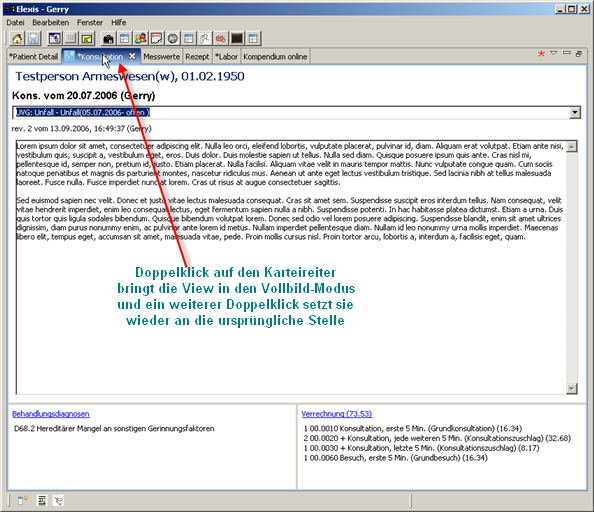
\includegraphics[width=0.9\textwidth]{images/tour3}
  \caption{View maximieren}
  \label{fig:tour3}
\end{center}
\end{figure}

\subsubsection{Aménager views et perspectives}


Dans la perspective de démarrage par défaut on trouve à gauche une \glqq barre de démarrage \grqq{}. Celle-ci vous amène à des perspectives prédéfinies dans lesquelles vous trouvez les affichages appropriés.
La barre d'outils mène, comme d'habitude pour d'autres programmes, à des différents fonctions. Chaque affichage a un onglet. Par un clic sur cet onglet l'affichage peut être mis au premier plan ou il peut être maximisé par un double clic comme déjà mentionné

\par
\clubpenalty=5000
\medskip
Le contenu des fenêtres du programme et les compilations des affichages peuvent être facilement adaptés à vos besoins:\\

\begin{itemize}
  \item Vous pouvez supprimer des affichages dont vous n'avez pas besoin pour gagner de la place pour les affichages restants.
	\item Vous pouvez agrandir ou réduire la taille des affichages à l'horizontale et à la verticale.
	\item Vous pouvez déplacer les affichages à n'importe quel endroit sur l'écran (en \glqq maintenant enfoncé\grqq{}la touche gauche de la souris sur l'onglet de l'affichage en question '=drag and drop'  )
\end{itemize}

Chaque composition peut être enregistré en tant que perspective - et reste en tant que telle
facilement accessible.


\subsection{Aménager et sauvegarder des perspectives}
\label{tour:customize}
Vous ne pouvez pas seulement créer une seule perspective, mais autant que vous voulez. Votre assistante médicale aura peut-être besoin d'une autre perspective que vous-même, par exemple, elle souhaite avoir l'agenda en plein écran. Vous même, vous pouvez utiliser des différentes perspectives, par exemple une pour les consultations et une autre pour la comptabilité ou si vous devez écrire un rapport.
Dans Elexis des nouvelles perspectives peuvent être composées facilement:\\

\bigskip

\textbf{Premier pas : Ouvrez l'affichage (les affichages) souhaité}\\

Cliquez dans le menu  \textsc{WINDOW - PERSPECTIVE sur OTHER}. Une boite de dialogue s'ouvre. Voir Fig. \ref{fig:cust1}.\\

\begin{figure}[htbp]
   \begin{minipage}{0.4\textwidth}
       \centering
       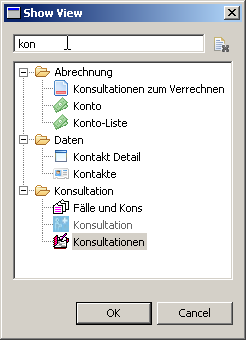
\includegraphics[width=0.8\textwidth]{images/customize1}
       \caption{View suchen}
       \label{fig:cust1}
     \end{minipage}\hfill
     \begin{minipage}{0.5\textwidth}
        Cette boîte de dialogue vous montre tous les affichages disponibles dans l'installation de votre Elexis. (Lesquels et combien ils sont est dépendant des plugins installés). La liste sera automatiquement filtrée, si vous tapez dans la première ligne de cette boite de dialogue le début du nom de l'affichage cherché.

        Si vous ne connaissez pas le nom de l'affichage cherché vous pouvez aussi parcourir tous les affichages.

    \end{minipage}
\end{figure}

\bigskip
\pagebreak[3]
\textbf{Deuxième pas : Déplacer les affichages à l'endroit souhaité et choisir sa taille :}\\

   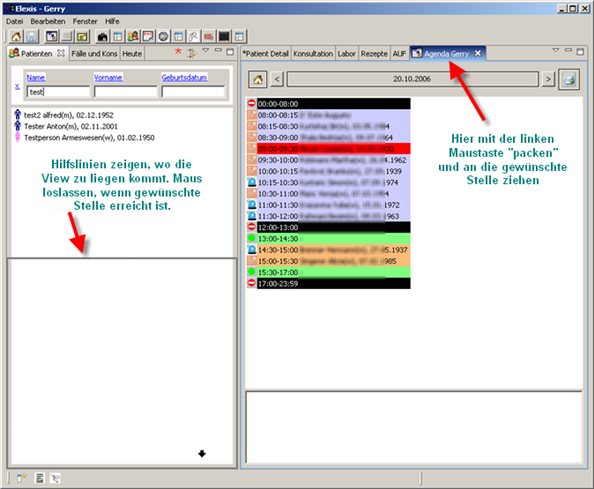
\includegraphics[width=0.8\textwidth]{images/agendagewaehlt}
Une ligne supplémentaire indique où l'affichage se trouvera. Relâchez la souris lorsque la position désirée est atteinte.
Saisir ici avec le bouton gauche de la souris et tirer à l'endroit souhaité. (drag and drop)
Si la flèche de la souris se trouve entre deux affichages (vertical ou horizontal), elle est est transformée en flèche double et peut ensuite déplacer la frontière entre les deux affichages.

   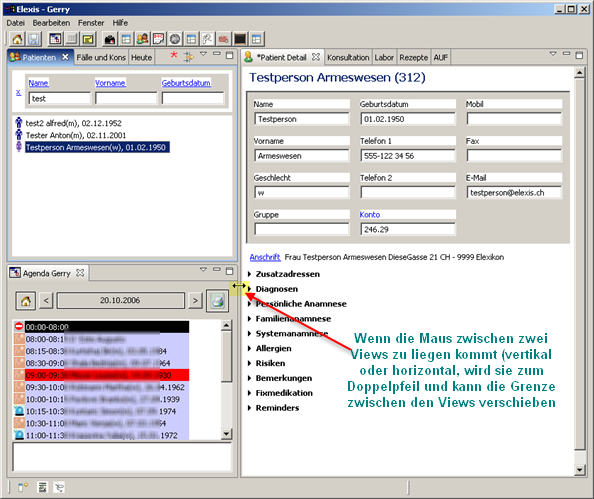
\includegraphics[width=0.8\textwidth]{images/agendaanpassen}

\bigskip
\textbf{Troisième pas : Sauvegarder la perspective}\\
\index{Sauvegarder la perspective}
Si vous souhaitez que votre perspective ainsi établi soit aussi disponible lors d'un démarrage ultérieure ou sur d'autres ordinateurs vous avez plusieurs possibilités :
\begin{itemize}
\item Sélectionnez dans le menu  \textsc{FENÊTRE - PERSPECTIVE - SAUVEGARDER COMME PERSPECTIVE DE DEPART}. Ainsi, vous déterminez que cette perspective apparaisse désormais lors du démarrage.
\item \textsc{FENÊTRE - PERSPECTIVE - SAUVEGARDER COMME …}. Vous avez ainsi la possibilité de sauvegarder la perspective actuelle sous un nom quelconque. Sachant le nom de la perspective, vous pouvez la récupérer à une date ultérieure avec  \textsc{FENÊTRE - PERSPECTIVE - AUTRES...}.
\item \textsc{FENÊTRE - PERSPECTIVE - SAUVEGARDER}. Dans ce cas la perspective actuelle est sauvegardée sous le nom actuel.
\item And last but not least : Si vous sauvegardez sous \textsc{FICHIER - REGLAGES - UTILISATEUR} la perspective sous un certain nom, vous pouvez l'utiliser aussi depuis un autre ordinateur sous le même nom\footnote{Ceci n'est naturellement possible que si sur le poste concerné tout les affichages existent, dont on aura besoin dans cette perspective}. Cette option est idéale pour créer un environnement de travail homogène.
\end{itemize}

\textbf{Ou : réinitialiser la perspective}\\
\index{réinitialiser la perspective}
Si les modifications ne vous conviennent quand même pas, ou si vous avez fermé
par exemple par erreur un affichage, vous pouvez tout simplement retourner
à la version de la perspective actuelle enregistrée : Choisissez dans le menu
\textsc{FENÊTRE - PERSPECTIVE - RECONSTITUER.} Ceci n'est naturellement possible que, tant que
vous n'avez pas stocké vos modifications.(troisième pas).


